% !TeX encoding = UTF-8
% !TeX root = V7_Lichtbeugung.tex
% !TeX spellcheck = de_DE_frami

% \section{Einleitung}


\newpage
\section{Theorie}
\subsection{Geometrische Optik}
Auf makroskopischer Ebene in einem homogenen Medium lässt sich eine elektromagnetische Lichtwelle als Strahl ausgehend von der Quelle beschreiben. Diese breitet sich in Richtung des Wellenvektors aus. Für den Strahlengang durch eine dünne konvexe Linse gilt die Linsengleichung
\begin{equation}
\frac{1}{f}=\frac{1}{g}+\frac{1}{b},
\label{eq:abb_gleichung}
\end{equation}

wobei $f$ die Brennweite der Linse, $g$ die Gegenstandsweite zur Linse, und $b$ der entsprechende Abstand zur Linse ist. Für $g=\infty$, dies entspricht einen Strahl parallel zur optischen Achse, ist $b=f$. Ist dagegen $b=\infty$, so gilt $g=f$. Damit lassen sich optische Abbildungen wie in Abbildung \ref{fig:geo_optik} konstruieren.

\begin{figure}[h]
	\centering
	\includegraphics[width=0.9\textwidth]{linsengleichung.pdf}
	\caption{Konstruktion einer Abbildung mit der Linsengleichung.}
	\label{fig:geo_optik}
\end{figure}

\newpage
\enlargethispage{3em}
\subsection{Abbildungsfehler}
Linsen sind im Allgemeinen nicht stigmatisch, d.h. ein Punkt der Gegenstandsebene wird nicht auf einen Punkt in der Bildebene abgebildet. Im folgenden lassen sich die Abbildungsfehler, die sogenannten \emph{Aberrationen}, grob in zwei Kategorien einteilen.

\subsubsection{Chromatische Aberration}		\vspace{-1ex}
Dieser Fehler beruht auf der wellenlängenabhängigen Brechungszahl $n(\lambda)$ (\emph{Dispersion}). Die Linse besitzt für verschiedene Wellenlängen unterschiedliche Foki, dies ist in Abbildung \ref{fig:chromatic_abb} veranschaulicht.
Beheben lässt sich die chromatische Aberrationen bei optischen Linsen durch das Anbringen eines \emph{Achromaten}, eine konkave Linse mit einer anormalen Dispersion.

\subsubsection{Monochromatische Aberrationen}	\vspace{-1ex}
Die Ursache dieser Aberrationen ist die Geometrie der {\marker durchlaufenen} Linse.

\begin{description}
\item[Sphärische Aberration] tritt bei sphärisch geschliffenen Linsen auf und hat als Ursache, dass achsenferne Strahlen nicht mehr der paraxialen Näherung genügen. Sie werden in einem anderen Brennpunkt fokussiert als achsennahe Strahlen (vgl. Abbildung \ref{fig:spheric_abb}), für welche die Abbildungsgleichung \eqref{eq:abb_gleichung} gilt.

Diese Aberration lässt sich minimieren durch
\begin{itemize} \itemsep-1ex
	\item Unterdrückung der achsenfernen Strahlen mit z.B. einer Lochblende. Jedoch treten so Intensitätsverluste auf;
	\item Verwendung einer plankonvexen Linse, deren konvexen Seite der Gegenstandsseite zugewandt ist;
	\item eine Kombination von Sammel- und Zerstreuungslinsen;
	\item speziell geschliffene asphärische Linsen.
\end{itemize}

\item[Astigmatismus] entsteht, wenn das Objekt sich nicht auf der optischen Achse, sondern versetzt davon befindet. Dadurch fallen die Strahlenbündel schräg in die Linse, und es ergeben sich unterschiedliche Brennweiten in der sogenannten \emph{Meridional-} (M) und \emph{Sagittalebene} (S), wie in Abbildung \ref{fig:astigmatismus} veranschaulicht wird.

\item[Koma] ist eine Überlagerung der sphärischen Aberration und des Astigmatismus. Strahlen, welche nicht achsenparallel in die Linse einfallen, werden unterschiedlich an der Linse gebrochen und in einem anderem Bildpunkt der Bildebene fokussiert. Bei sphärischen Linsen entstehen dadurch Ringe, welche einen Schweif bilden (lat. \emph{coma}). Dies ist in Abbildung \ref{fig:koma} veranschaulicht. Die Koma kann durch Ausblenden achsenferner Strahlen gemildert werden, jedoch bleibt so der Astigmatismus schiefer Bündel bestehen.
\end{description}

\newpage
\begin{figure}[ht]
	\centering
	\begin{subfigure}[b]{0.45\textwidth}
		\centering
		\includegraphics[width=\textwidth]{chromatic_abb.pdf}
		\caption{Chromatische Aberration}
		\label{fig:chromatic_abb}
	\end{subfigure}
	\hfill
	\begin{subfigure}[b]{0.45\textwidth}
		\centering
		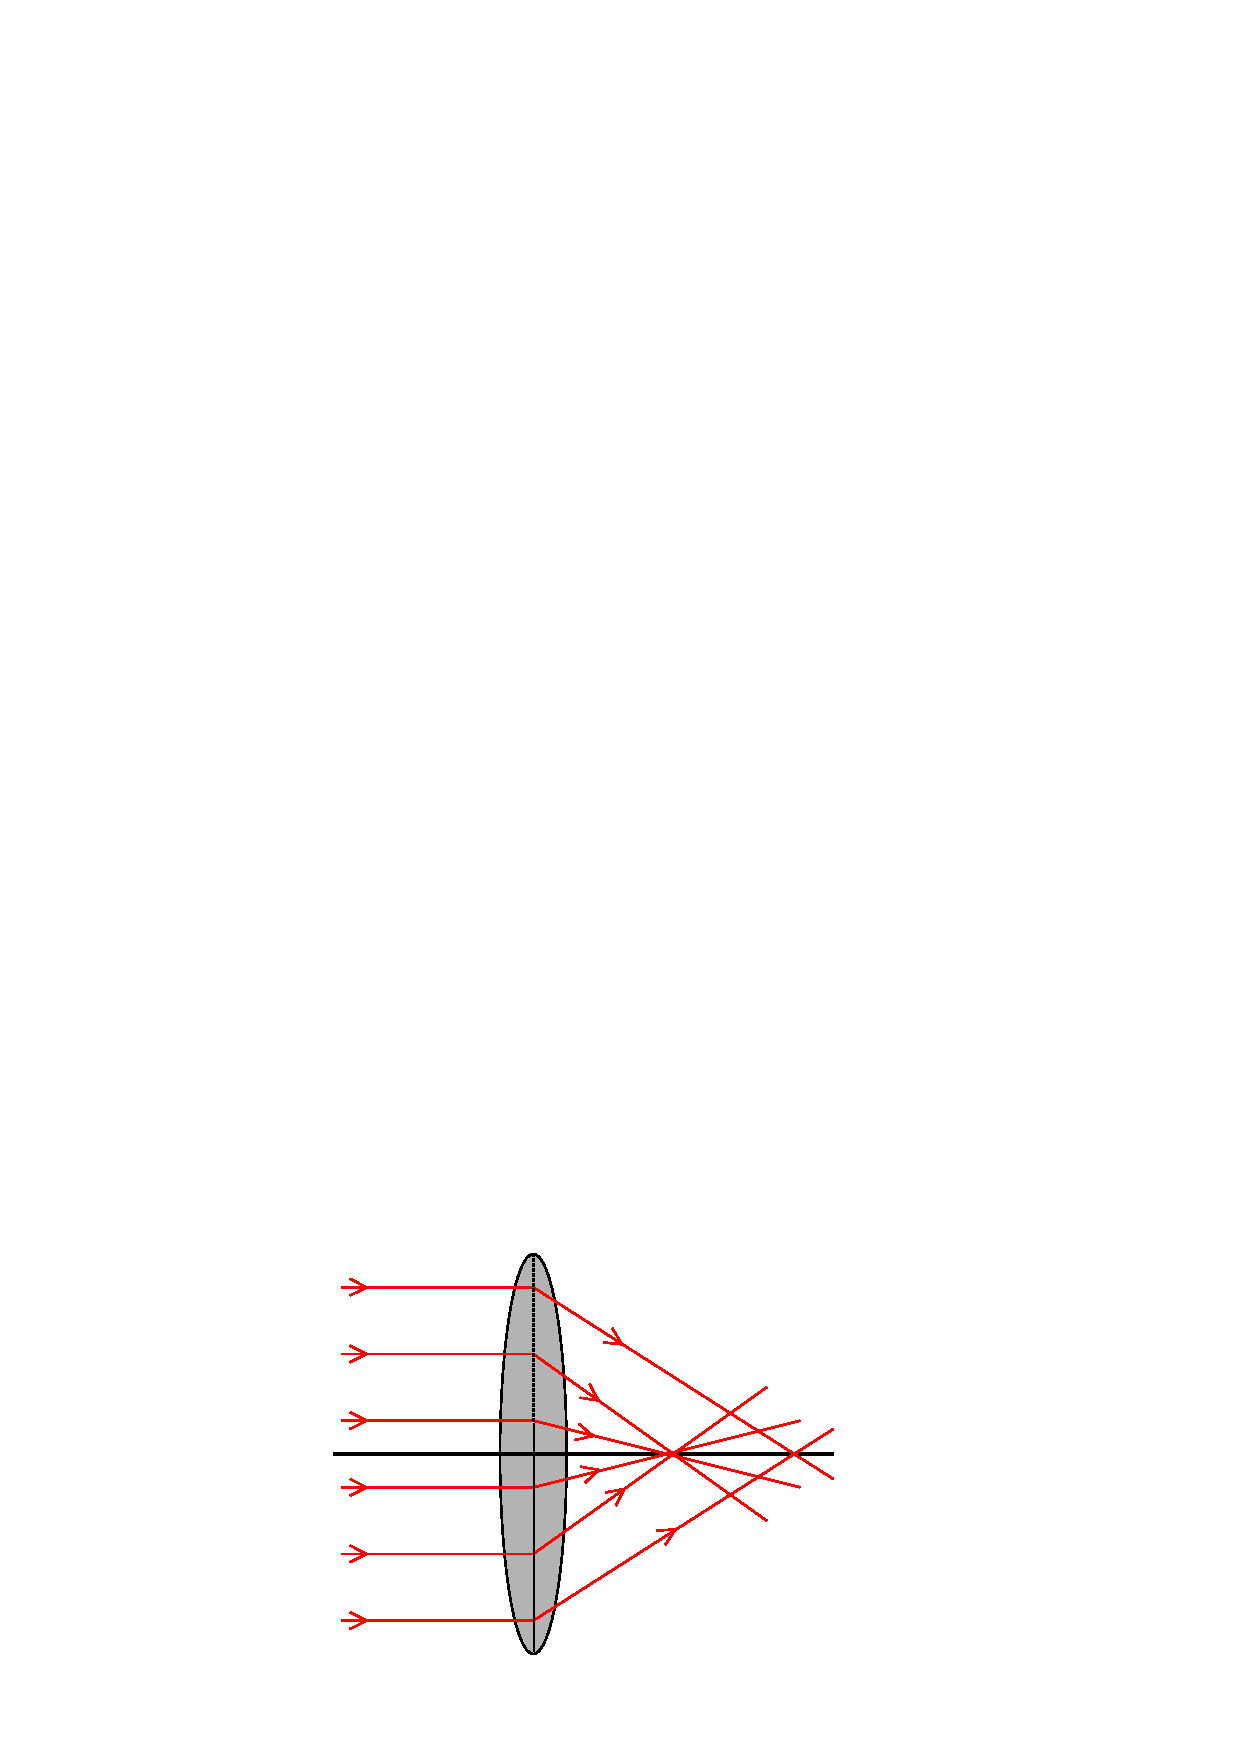
\includegraphics[width=\textwidth]{spheric_abb.pdf}
		\caption{\marker Sphärische Aberration}
		\label{fig:spheric_abb}
	\end{subfigure}
	
	\begin{subfigure}[b]{0.45\textwidth}
		\centering
		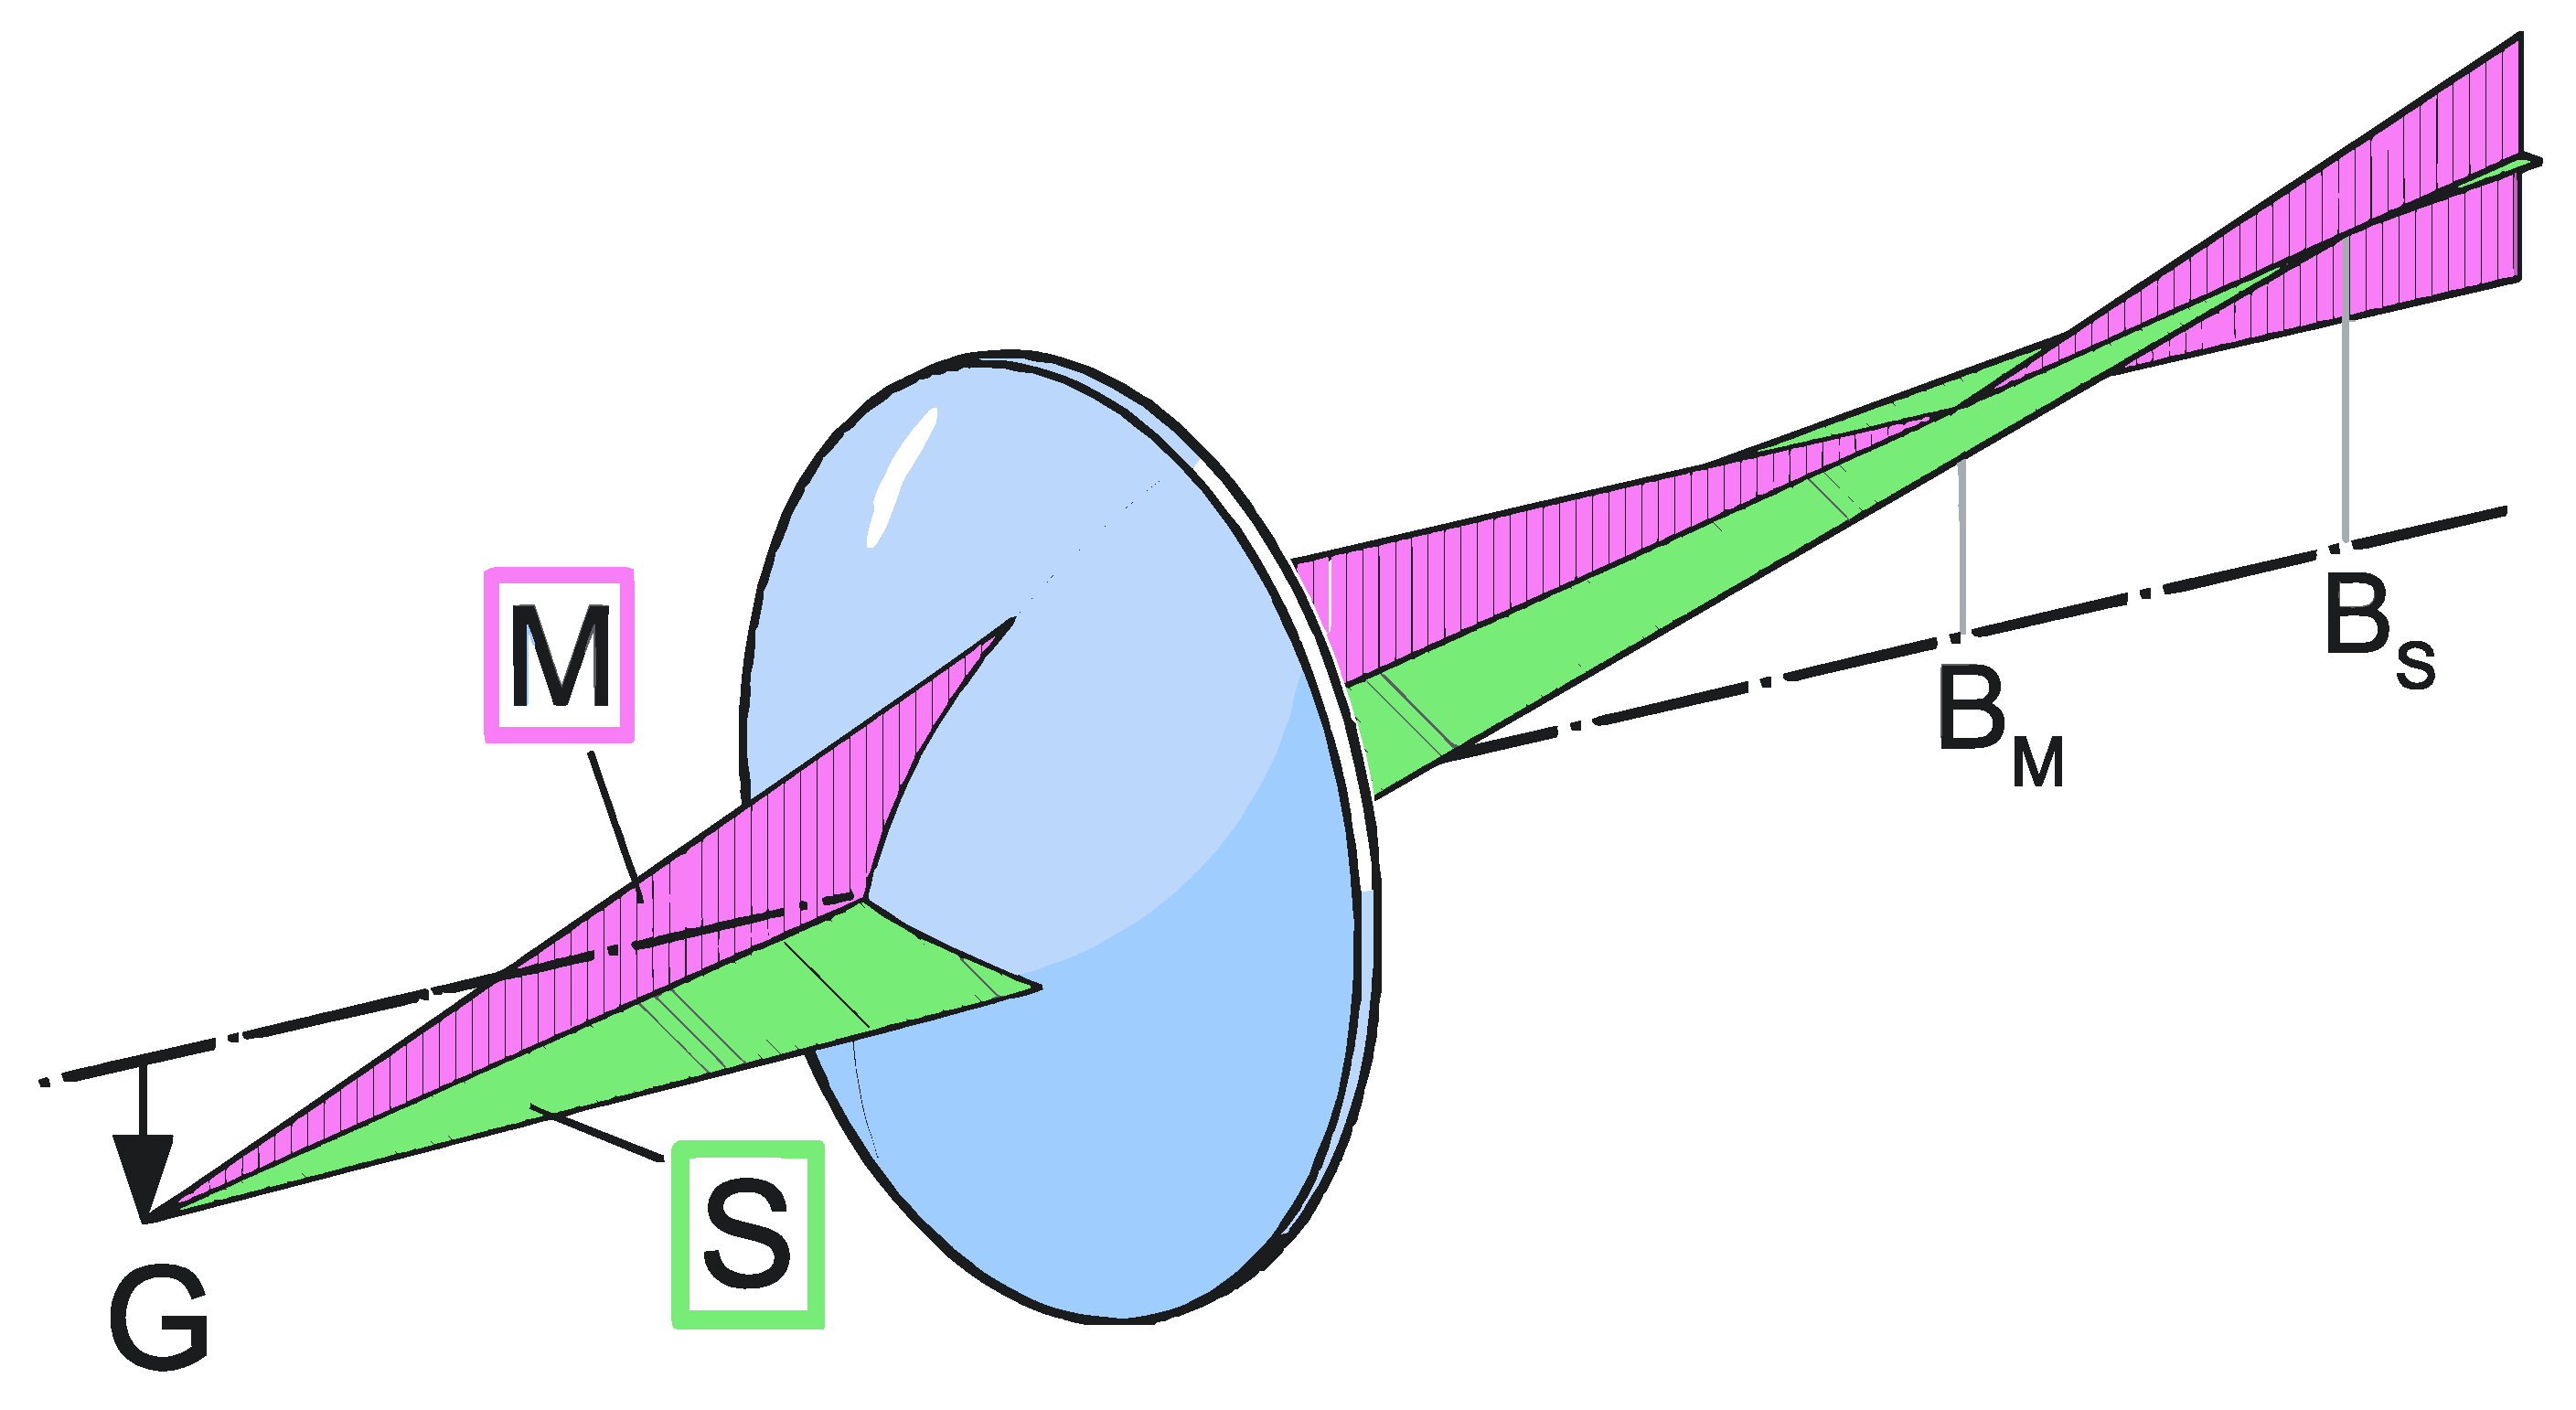
\includegraphics[width=\textwidth]{Meridional_SagittalPlane.pdf}
		\caption{Astigmatismus \cite{lit:wiki_astigma}}
		\label{fig:astigmatismus}
	\end{subfigure}
	\hfill
	\begin{subfigure}[b]{0.45\textwidth}
		\centering
		\includegraphics[width=\textwidth]{koma.pdf}
		\caption{\marker Koma}
		\label{fig:koma}
	\end{subfigure}
	\caption{Abbildungsfehler in der geometrischen Optik.}
%	\vspace{-3em}
\end{figure}

\subsection{Wellenoptik}
Das Huygenssche Prinzip interpretiert Licht als Welle. Jeder Punkt der Wellenfront zum Zeitpunkt $t$ ist Quelle einer neuen Elementarwelle (im Vakuum eine Kugelwelle), deren Überlagerung in $t + \d t$ eine neue Wellenfront bildet. Ebene Wellenfronten breiten sich gleichmäßig aus, weshalb ihr Normalenvektor erhalten bleibt -- dies ist die Grundlage der Strahlenoptik. Allerdings ermöglicht die Wellenoptik zusätzlich die Beschreibung von Phänomenen am Rand der Welle (\emph{Beugung}) sowie die Überlagerung von Wellen (\emph{Interferenz}).

Wir betrachten im Folgenden die Beugung der elektromagnetischen Welle an einem Objekt.

\subsubsection{Kirchhoffsches Beugungsintegral}
Für jede Elementarwelle gilt die Energieerhaltung
\begin{equation}
W(r) = \iint\limits_\text{Kugel}\!\! I \;\d A = E^2 \cdt 4 \pi r^2 = \const = W(0)
\end{equation}
und somit $|E(r)| = \frac{E(0)}{r}$. Die Phasenverschiebung ist durch den Wellenvektor $\vec k$ gegeben als $e^{i n \vec k \vec r}$.

Integrieren wir über alle Punkt-Quellen $P_1 (x_1, y_1, 0)$ einer Blende, so ergibt sich für die Feldstärke in einem Punkt $P_2 (x_2, y_2, z_2)$
\begin{equation}
E(P_2) = \iint\limits_\text{Blende}\!\! E(P_1) \cdot \frac{e^{i n \vec k \vec r_{12}}}{r_{12}} \;\d A		\label{eq:kirchhoff1}
\end{equation}

Gleichung \eqref{eq:kirchhoff1} genügt, um die Beugung einer ebenen Welle zu beschreiben. Für die Abbildung eines Objektes in $P_0 (0, 0, -z_0)$ vor der Blende\footnote{Zur Vereinfachung wählen wir unser Koordinatensystem so, dass $P_0$ auf der optischen Achse liegt.} muss zusätzlich $E(P_1)$ berechnet werden. Sei $\alpha_{ij}$ der Winkel von $\vec r_{ij}$ zur optischen Achse und $k_{ij} = k \sin \alpha_{ij}$ die Projektion von $k$ auf $\vec r_{ij}$, so gilt \cite[S.\,30]{lit:HL-Laser}
\begin{equation}
E(P_1) = \frac{n}{i\lambda} E(P_0) \frac{e^{i n k_{01} r_{01}}}{r_{01}} \cdt \frac{\cos \alpha_{01} + \cos \alpha_{12}}{2}
\end{equation}

Da wir im folgenden jedoch unsere Blende mit parallelem Licht abbilden, rechnen wir im Folgenden mit Gleichung \eqref{eq:kirchhoff1} weiter.

\subsubsection{Fresnel-Beugung}
Sei $r_{12} \approx z_2$ (Nahfeld bis Fernfeld) und der radiale Abstand $\rho^2 := (x_2 - x_1)^2 + (y_2 - y_1)^2$, so genügt die Taylor-Näherung 
\begin{equation}
r_{12} = \sqrt{z_2^2 + \rho^2} = z_2 \cdt \left( 1 + \tfrac{\rho^2}{2 z_2^2} + \mathcal{O}(\tfrac{\rho^4}{z_2^4}) \right)
\end{equation}

In Gleichung \eqref{eq:kirchhoff1} eingesetzt erhalten wir die Fresnel-Näherung
\begin{equation}
E(P_2) = \frac{e^{i n k z_2 }}{z_2} \iint\limits_\text{Blende}\!\! E(P_1) \cdot e^{i n k_{12} \frac{\rho^2}{2 z_2} } \;\d A
\label{eq:Fresnel_B}
\end{equation}

\subsubsection{Fraunhofer Beugung}
Ist zudem $z_2 \gg k \rho^2$, also die Blende deutlich kleiner als der Abstand zur Bildebene, so genügt die erste Ordnung in $x_1$ und $y_1$
\begin{equation}
\rho^2 ~\approx~ x_2^2 + y_2^2 - x_1 x_2 - y_1 y_2
\end{equation}
 und das Beugungsintegral vereinfacht sich zur Fraunhofer-Näherung:
\begin{equation}
E(P_2) =  \underbrace{
\frac{1}{z_2} \exp \left(i n k (z_2 +  \tfrac{x_2^2 + y_2^2}{2 z_2}) \right)
}_{A(x_2, y_2, z_2)} ~
\iint\limits_\text{Blende}\!\! E(P_1) \cdot e^{-i n k_{12} \frac{x_1 x_2 + y_1 y_2}{2 z_2} } \;\d x_1 \d y_1
\end{equation}

Weiterhin lässt sich die Form der Blende durch die Transmissionsfunktion $\tau$ darstellen:
\begin{equation}
\tau(x_1, y_1) := \mathds{1} \bigl[(x_1, y_1) \in \text{Blende} \bigr]
\iff	\!\iint\limits_\text{Blende}\!\!\! f \;\d x_1 \d y_1 = \Fint[\iint] f ~ \tau(x_1, y_1) \;\d x_1 \d y_1
\end{equation}

Nehmen wir an, dass die Feldstärkenverteilung $E(P_1)$ homogen und normalisiert ist, und lassen $A(x_2,y_2,z_2)$ kurz außer Betracht, so stellt sich heraus, dass die Fraunhofer Beugung die Fouriertransformation von $\tau$, also der Form des beugenden Objekts, ist:
\begin{equation}
\mathcal{F}[\tau(x)](k) := \Fint \tau(x) e^{ikx} \;\d x
\qquad
\mathcal{F}^{-1}[g(k)](x) := \tfrac{1}{2 \pi} \Fint g(k) e^{-ikx} \;\d k
\end{equation}
Somit lassen sich die Beugungsbilder verschiedener Objekte berechnen. Dazu ist das folgende Theorem sehr nützlich.


\begin{figure}[h]
	\centering
	\vspace{1ex}
	\def\svgwidth{0.75\textwidth}
	\input{graphics/NahFern.pdf_tex}
	\caption{Beugungsbild eines Einzelspalts im Nah- und Fernfeld \cite[S.\,342]{lit:DR}}
	\vspace{-3em}
\end{figure}

\subsubsection{Faltungstheorem}
Für zwei Funktionen $f(x)$ und $g(x)$ ist die Faltung $(f*g)(x)$ definiert mit
\begin{align}
(f*g)(x)=\Fint f(t)g(x-t)~\d t.
\end{align}
Für die Fouriertransformierte $\mathcal{F}[~](k)$ der Faltung gilt dann
\begin{align}
\mathcal{F}[(f*g)(x)](k)=\mathcal{F}[f(x)](k)\cdt \mathcal{F}[g(x)](k).
\end{align}
Durch Einsetzen der inversen Fouriertransformierten lässt sich ebenso zeigen, dass gilt:
\begin{align}
\mathcal{F}[f(x)](k)* \mathcal{F}[g(x)](k)=\mathcal{F}[(f\cdt g)(x)](k).
\end{align}
Damit lassen sich u.a. Beugungsbilder von Objekten, die einer Modulierung unterliegen, wesentlich einfacher berechnen.


\subsubsection{Babinetsches Prinzip}
Das Babinetsche Prinzip besagt, dass die Summe der Felder $E, E'$ die durch die Beugung an komplementären Blenden $\tau, \tau' = 1-\tau$ entstehen, der einfallenden Welle entspricht. Anschaulich erklärt ergänzen sich die Blenden zu einer vollen durchlässigen Ebene, weshalb keine Beugung auftritt.


\subsubsection{Fresnel-Zonen}
Betrachten wir erneut den Aufbau zu Gleichung \eqref{eq:Fresnel_B} und fordern, dass $x_2 = y_2 = 0$ und $E(P_1)$ homogen seien. Teilwellen mit einer Phasenverschiebung $n k \frac{\rho^2}{2 z_2} \in [-\tfrac\pi2, \tfrac\pi2 ]$ interferieren konstruktiv, jene mit $[\tfrac\pi2, \tfrac32 \pi ]$ destruktiv.
Somit lässt sich die Objektebene in ringförmige Zonen unterteilen, die abwechselnd positiv bzw. negativ zur Feldstärke in $P_2$ beitragen:
\begin{equation}
\rho_m^2 =  \frac{m \cdt 2 z_2 \cdt \pi}{n k} = m z_2 \lambda
\iff \rho_m = \sqrt{m z_2 \lambda}
\end{equation}

Eine Fresnelsche Zonenplatte ist eine Blende aus Ringen, welche alle ungeradzahligen Zonen ($\rho_1 \to \rho_2, \rho_3 \to \rho_4, \dots$) ausblenden. Somit treten in $P_2$ nur positive Beiträge zur Feldstärke auf, weshalb die Zonenplatte das Licht dort bündelt und den Effekt einer Linse hat.



\subsubsection{Berechnung von Beugungsbildern}
\enlargethispage{2em}
Zunächst berechnen wir die Fouriertransformierten $\mathcal{F}[\tau(x)](k)$ verschiedener eindimensionaler Funktionen:
\begin{align}
\mathcal{F}[1](k)
&= \Fint e^{ikx} \d x = \delta(k)
\\[1em]
\mathcal{F}[\delta(x)](k)
&= \Fint \delta(x) e^{ikx} \d x
  = \left. e^{ikx} \right|_{x=0} =  1
\\[1em]
\mathcal{F}\bigl[\delta(x\!-\!\tfrac{d}{2}) + \delta(x\!+\!\tfrac{d}{2})\bigr](k)
&%= \Fint \delta(x\!-\!\tfrac{d}{2}) e^{ikx} \d x + \Fint \delta(x\!+\!\tfrac{d}{2}) e^{ikx} \d x
  = e^{ik \frac d2} + e^{-ik \frac d2} = 2 \cos(k \; \tfrac d2)
\label{eq:doppel}		\\[1em]
\mathcal{F}\left[\sum\limits_{n=0}^{N-1} \delta(x-ng) \right](k)
&= \Fint \sum\limits_{n=0}^{N-1} \delta(x-ng) e^{-ikx}\d x
  =\sum\limits_{n=-0}^{N-1} e^{-ikng}												\nonumber\\
&= \frac{e^{-ikNg}-1}{e^{-ikg}-1}
  = \exp \bigl(-\tfrac12 ikg(N\!-\!1) \bigr) \cdt \frac{\sin(\tfrac12 kNg)}{\sin(\tfrac12 kg)}			%\\
% \xrightarrow{N \to \infty}&~ \frac{1}{1 - e^{-ikg}}
% \tfrac12- \tfrac1/2 i \cot(\tfrac{x}{2}) ???
\label{eq:kamm}		\\[1em]
\mathcal{F}\left[\Theta\bigl(\tfrac{b}{2}-|x|\bigr) \right](k)
&= \Fint \Theta\bigl(\tfrac{b}{2}-|x|\bigr) e^{ikx} \d x
  = \int\limits_{-b/2}^{b/2} e^{ikx} \d x = \left. \frac{e^{ikx}}{ik} \right|_{-b/2}^{b/2}					\nonumber\\
&= \frac{e^{\frac12 ikb} - e^{-\frac12 ikb}}{2i \cdt \tfrac12 k}
  = b ~ \frac{\sin \tfrac12 kb}{\tfrac12 kb}
  = b \; \sinc \tfrac12 kb
\label{eq:rechteck}	\\[1em]
\mathcal{F}[\sin(x)](k)
&= \Fint \frac{e^{ix}-e^{-ix}}{2i} e^{ikx} \d x
%  = \left. \frac{e^{i(k-1)x}}{2(k-1)} - \frac{e^{i(k+1)x}}{2(k+1)} \right|_{-\infty}^{\infty}				\nonumber\\
  = i \pi \delta(k-1) - i \pi \delta(k+1)
\\[1em]
\mathcal{F}[\cos(x)](k)
&= \Fint \frac{e^{ix}+e^{-ix}}{2} e^{ikx} \d x
%  = \left. \frac{e^{i(k-1)x}}{2(k-1)} - \frac{e^{i(k+1)x}}{2(k+1)} \right|_{-\infty}^{\infty}				\nonumber\\
  = \pi \delta(k-1) + \pi \delta(k+1)
\\[1em]
\mathcal{F}\left[\exp\bigl(-\frac{x^2}{2 \sigma^2}\bigr)\right](k)
&= \Fint\! \exp\bigl(-\frac{x^2}{2 \sigma^2} + ikx\bigr) \,\d x
  = e^{-\frac12 k^2\sigma^2} \!\Fint \exp{-\frac12 \bigl( \frac{x}{\sigma} - ik\sigma \bigr)^2} \,\d x		\nonumber\\
&= \sigma \; e^{-\frac12 k^2\sigma^2} \!\Fint e^{-\frac12 u^2} \d u
  = \sqrt{2\pi} \; \sigma \cdt e^{-\frac12 k^2\sigma^2}
\end{align}


\subsubsection*{Beugung am Einzelspalt}
Für einen Einzelspalt der Breite $b$ ist die Transmissionsfunktion $\tau(x,y) = \Theta\bigl(\tfrac{b}{2}-|x|\bigr) \cdt 1$, folglich gilt für das Beugungsbild Gleichung\eqref{eq:rechteck}.

Die Intensitäts-Minima im Beugungsmuster treten auf für 
\begin{equation}
\sinc \tfrac12 kb = 0
\iff \tfrac12 kb = m \pi,~ m \in \mathds{Z}/\{0\}
\iff b \sin \alpha_{12} = m \lambda
\end{equation}
Hierbei nutzen wir $k_{12} = k_z \sin \alpha_{12} = \frac{2 \pi}{n \lambda} \sin \alpha_{12}$.

Im späteren Versuchsaufbau bilden wir das Beugungsbild mit $g=\infty$ durch eine Linse mit Brennweite $f$ in deren Brennebene ab; aufgrund des Mittelpunktstrahls ist der Winkel von der Linse zum Bildpunkt ebenfalls $\alpha_{12}$. Für die Positionen $(0, y_S, f)$ auf dem Schirm relativ zur Linse gilt folglich
\begin{equation}
\tan \alpha_{12} = \tfrac{y_S}{f} 	\iff	 \alpha_{12} = \arctan \tfrac{y_S}{f}
\end{equation}

Die Spaltbreite lässt sich also anhand der Position der Minima auf dem Schirm bestimmen:
\begin{equation}
b = m \lambda \div \sin \left(\arctan \tfrac{y_S}{f}\right)
\label{eq:Messung}
\end{equation}

\subsubsection*{Beugung am Doppelspalt}
Da sich ein Doppelspalt aus zwei Einzelspalten im Abstand $d$ zusammensetzt, erhalten wir mit \eqref{eq:doppel} über das Faltungstheorem
\begin{equation}
\mathcal{F}[\tau(x)](k) =
b \sinc \tfrac12 kb \cdot \cos \tfrac12 kd
\end{equation}


\subsubsection*{Beugung am Gitter}
Ein ideales Gitter lässt sich durch einen Delta-Kamm \eqref{eq:kamm} als Transmissionsfunktion beschreiben. Berücksichtigen wir die endliche Spaltbreite $b$ eines realen Gitters, so entspricht dies der Faltung mit der Rechteckfunktion \eqref{eq:rechteck}.
Die Fouriertransformierte ist entsprechend
\begin{equation}
\mathcal{F}[\tau(x)](k) =
b ~ \exp \bigl(-\tfrac12 ikg(N\!-\!1) \bigr) \cdt \frac{\sin(\tfrac12 kNg)}{\sin(\tfrac12 kg)} ~ \sinc \tfrac12 kb
\end{equation}




%
%\begin{figure}[p]
%	% !TeX root = ../../V7_Lichtbeugung.tex
\begin{tikzpicture}

\begin{axis}[%
width=0.95\textwidth,
height=0.5\textwidth,
xmin=-pi,
xmax=pi,
xlabel={$x$},
ymin=-1.1,
ymax=1.1,
extra y ticks = 0,
extra y tick style = {grid=major}
% ylabel={$y$ bzw. $y \div i \pi$},
]
\addplot [samples=500, color=black]
plot (\x, {sin(360 * \x / (2*pi)});

\addplot [ycomb, color=red]
plot coordinates {(-1,-1) (1,1)};

\end{axis}
\end{tikzpicture}%
%	% !TeX root = ../../V7_Lichtbeugung.tex
\begin{tikzpicture}

\begin{axis}[%
width=0.95\textwidth,
height=0.5\textwidth,
at={(0\textwidth,0\textwidth)},
%scale only axis,
xmin=-5,
xmax=5,
xlabel={$\tfrac{x}{\sigma}$ bzw. $\sigma k$},
ymin=0,
ymax=1,
% ylabel={$y$ bzw. $y \div \sqrt{2\pi}\sigma$}
]
\addplot [samples=500, color=black]
plot (\x, {exp(-pow(\x,2) / 2)});

\addplot [samples=500, color=red]
plot (\x, {exp(-pow(\x,2))});

\end{axis}
\end{tikzpicture}%
%\end{figure}


